% !TEX program = pdflatex
% Compile this handout from the repository root with make problems.
\documentclass[nohyper,nobib,nofonts]{tufte-handout}
% Shared packages and typography for the book and homework handouts.
\usepackage[T1]{fontenc}
% Give titletoc a separate part number before nameref wraps \@part.
\usepackage{etoolbox}
\makeatletter
\@ifclassloaded{tufte-book}{%
  \patchcmd{\@part}
    {\thepart\hspace{1em}}
    {\protect\numberline{\thepart}}
    {}
    {\PackageError{analysis-notes}{Could not format part contents labels}
      {Check the book class definition of \string\@part.}}
}{}
\makeatother
\usepackage{nameref}
\usepackage{amsmath,amssymb,amsthm}
\usepackage{graphicx}
\usepackage{booktabs}
% Packages used by the temporary Tufte specimen content.
\usepackage{fancyvrb,xspace,units,multicol,makeidx}
\fvset{fontsize=\small}
\usepackage{url}
\usepackage{lipsum} % Remove after all placeholder prose has been replaced.
\usepackage[backend=biber,natbib=true,style=numeric]{biblatex}
\addbibresource{bibliography.bib}

% Preserve the template's full citations in the margin.
\usepackage{xargs}
\renewcommandx{\cite}[3][1={0pt},2={}]{\sidenote[][#1]{\fullcite[#2]{#3}}}

\graphicspath{{figures/}}
\setkeys{Gin}{width=\linewidth,totalheight=\textheight,keepaspectratio}
\setcounter{secnumdepth}{1}

% Retain the borrowed title/contents design only for the book.
% Adapted from Kevin Godby's Tufte-LaTeX title/contents example:
% https://groups.google.com/forum/#!topic/tufte-latex/ujdzrktC1BQ
\makeatletter
\@ifclassloaded{tufte-book}{%
  \makeindex
  \setcounter{tocdepth}{0} % Parts and chapters only.
  % Title-only chapter headings; retain counters for sections and references.
  \titleformat{\chapter}[block]
    {\relax\ifthenelse{\NOT\boolean{@tufte@symmetric}}{\begin{fullwidth}}{}}
    {}
    {0pt}
    {\huge\rmfamily\itshape}
    [\ifthenelse{\NOT\boolean{@tufte@symmetric}}{\end{fullwidth}}{}]
  \renewcommand{\maketitlepage}{%
    \begingroup
    \setlength{\parindent}{0pt}
    {\fontsize{24}{24}\selectfont\textit{\@author}\par}
    \vspace{1.75in}
    \begin{fullwidth}
      \raggedright
      {\fontsize{36}{44}\selectfont\@title\par}
    \end{fullwidth}
    \vspace{0.5in}
    {\fontsize{14}{14}\selectfont\textsf{\smallcaps{\@date}}\par}
    \vfill
    {\fontsize{14}{14}\selectfont\textit{\@publisher}\par}
    \thispagestyle{empty}
    \endgroup
  }
  \titlecontents{part}
    [0pt]
    {\addvspace{0.75\baselineskip}\normalfont\normalsize}
    {\allcaps{Part~\thecontentslabel}\quad\allcaps}
    {\allcaps}
    {}
    [\vspace{0.5\baselineskip}]
  % Hide chapter numbers in the contents as well.
  \titlecontents{chapter}
    [4em]
    {\normalfont\normalsize}
    {\textit}
    {\textit}
    {\qquad\thecontentspage}
    [\vspace{0.5\baselineskip}]
}{}
\makeatother

% Shared notation and environments. Keep topic-specific macros local.
\newcommand{\N}{\mathbb{N}}
\newcommand{\Z}{\mathbb{Z}}
\newcommand{\Q}{\mathbb{Q}}
\newcommand{\R}{\mathbb{R}}
\newcommand{\C}{\mathbb{C}}

% Publication month and year used on the copyright page.
\newcommand{\monthyear}{%
  \ifcase\month\or January\or February\or March\or April\or May\or June\or
  July\or August\or September\or October\or November\or December\fi
  \space\number\year
}

% One shared counter makes results unambiguous within each section.
\theoremstyle{plain}
\newtheorem{theorem}{Theorem}[section]
\newtheorem{lemma}[theorem]{Lemma}
\newtheorem{proposition}[theorem]{Proposition}
\newtheorem{corollary}[theorem]{Corollary}
\theoremstyle{definition}
\newtheorem{definition}[theorem]{Definition}
\newtheorem{example}[theorem]{Example}
\newtheorem{exercise}[theorem]{Exercise}
\theoremstyle{remark}
\newtheorem{remark}[theorem]{Remark}

% BEGIN TUFTE PLACEHOLDER HELPERS
% Adapted from the supplied Tufte-LaTeX sample (Apache-2.0).
% Remove these documentation helpers once the specimens are replaced.
\newcommand{\hangp}[1]{\makebox[0pt][r]{(}#1\makebox[0pt][l]{)}}

%%
% Prints an asterisk that takes up no horizontal space.
% Useful in tabular environments.

%%
% Prints a trailing space in a smart way.


%%
% Some shortcuts for Tufte's book titles.  The lowercase commands will
% produce the initials of the book title in italics.  The all-caps commands
% will print out the full title of the book in italics.
\newcommand{\vdqi}{\textit{VDQI}\xspace}
\newcommand{\ei}{\textit{EI}\xspace}
\newcommand{\ve}{\textit{VE}\xspace}
\newcommand{\be}{\textit{BE}\xspace}
\newcommand{\VDQI}{\textit{The Visual Display of Quantitative Information}\xspace}
\newcommand{\EI}{\textit{Envisioning Information}\xspace}
\newcommand{\VE}{\textit{Visual Explanations}\xspace}
\newcommand{\BE}{\textit{Beautiful Evidence}\xspace}

\newcommand{\TL}{Tufte-\LaTeX\xspace}

% Typesets the font size, leading, and measure in the form of 10/12x26 pc.
\newcommand{\measure}[3]{#1/#2$\times$\unit[#3]{pc}}

% Macros for typesetting the documentation
\newcommand{\hlred}[1]{\textcolor{Maroon}{#1}}% prints in red
\newcommand{\hangleft}[1]{\makebox[0pt][r]{#1}}
\newcommand{\hairsp}{\hspace{1pt}}% hair space
\newcommand{\hquad}{\hskip0.5em\relax}% half quad space
\newcommand{\ie}{\textit{i.\hairsp{}e.}\xspace}
\newcommand{\eg}{\textit{e.\hairsp{}g.}\xspace}
\newcommand{\na}{\quad--}% used in tables for N/A cells
\providecommand{\XeLaTeX}{X\lower.5ex\hbox{\kern-0.15em\reflectbox{E}}\kern-0.1em\LaTeX}
\newcommand{\tXeLaTeX}{\XeLaTeX\index{XeLaTeX@\protect\XeLaTeX}}
% \index{\texttt{\textbackslash xyz}@\hangleft{\texttt{\textbackslash}}\texttt{xyz}}
\newcommand{\tuftebs}{\symbol{'134}}% a backslash in tt type in OT1/T1
\newcommand{\doccmdnoindex}[2][]{\texttt{\tuftebs#2}}% command name -- adds backslash automatically (and doesn't add cmd to the index)
\newcommand{\doccmddef}[2][]{%
  \hlred{\texttt{\tuftebs#2}}\label{template:cmd:#2}%
  \ifthenelse{\isempty{#1}}%
    {% add the command to the index
      \index{#2 command@\protect\hangleft{\texttt{\tuftebs}}\texttt{#2}}% command name
    }%
    {% add the command and package to the index
      \index{#2 command@\protect\hangleft{\texttt{\tuftebs}}\texttt{#2} (\texttt{#1} package)}% command name
      \index{#1 package@\texttt{#1} package}\index{packages!#1@\texttt{#1}}% package name
    }%
}% command name -- adds backslash automatically
\newcommand{\doccmd}[2][]{%
  \texttt{\tuftebs#2}%
  \ifthenelse{\isempty{#1}}%
    {% add the command to the index
      \index{#2 command@\protect\hangleft{\texttt{\tuftebs}}\texttt{#2}}% command name
    }%
    {% add the command and package to the index
      \index{#2 command@\protect\hangleft{\texttt{\tuftebs}}\texttt{#2} (\texttt{#1} package)}% command name
      \index{#1 package@\texttt{#1} package}\index{packages!#1@\texttt{#1}}% package name
    }%
}% command name -- adds backslash automatically
\newcommand{\docopt}[1]{\ensuremath{\langle}\textrm{\textit{#1}}\ensuremath{\rangle}}% optional command argument
\newcommand{\docarg}[1]{\textrm{\textit{#1}}}% (required) command argument
\newenvironment{docspec}{\begin{quotation}\small\ttfamily\parskip0pt\parindent0pt\ignorespaces}{\end{quotation}}% command specification environment
\newcommand{\docenv}[1]{\texttt{#1}\index{#1 environment@\texttt{#1} environment}\index{environments!#1@\texttt{#1}}}% environment name
\newcommand{\docenvdef}[1]{\hlred{\texttt{#1}}\label{template:env:#1}\index{#1 environment@\texttt{#1} environment}\index{environments!#1@\texttt{#1}}}% environment name
\newcommand{\docpkg}[1]{\texttt{#1}\index{#1 package@\texttt{#1} package}\index{packages!#1@\texttt{#1}}}% package name
\newcommand{\doccls}[1]{\texttt{#1}}% document class name
\newcommand{\docclsopt}[1]{\texttt{#1}\index{#1 class option@\texttt{#1} class option}\index{class options!#1@\texttt{#1}}}% document class option name
\newcommand{\docclsoptdef}[1]{\hlred{\texttt{#1}}\label{template:clsopt:#1}\index{#1 class option@\texttt{#1} class option}\index{class options!#1@\texttt{#1}}}% document class option name defined
\newcommand{\docmsg}[2]{\bigskip\begin{fullwidth}\noindent\ttfamily#1\end{fullwidth}\medskip\par\noindent#2}
\newcommand{\docfilehook}[2]{\texttt{#1}\index{file hooks!#2}\index{#1@\texttt{#1}}}
\newcommand{\doccounter}[1]{\texttt{#1}\index{#1 counter@\texttt{#1} counter}}
% END TUFTE PLACEHOLDER HELPERS


\title{Homework 01}
\author{Introduction to Mathematical Analysis I}
\date{}

\begin{document}
\maketitle

\marginnote{\textit{Student}: Lucas Barbosa\\ \texttt{lc6424}}
\section{Sets and foundations}
\label{sec:hw01:sets-and-foundations}

We use $\N=\{1,2,3,\ldots\}$. A set is countable if it is finite
or countably infinite.

\begin{exercise}
\label{ex:hw01:de-morgan}
Let $\{A_\gamma \mid \gamma \in \Gamma\}$ be a collection of sets. Prove De Morgan's laws
\[
    \begin{aligned}
      \left(\bigcup_{\gamma\in\Gamma} A_\gamma\right)^c
        &= \bigcap_{\gamma\in\Gamma} A_\gamma^c,\\
      \left(\bigcap_{\gamma\in\Gamma} A_\gamma\right)^c
        &= \bigcup_{\gamma\in\Gamma} A_\gamma^c.
    \end{aligned}
\]
\end{exercise}


% Transcribed from IMG_8995 and the left page of IMG_8996.
\begin{proof}[Solution]
  Fix a set $S$ such that $A_\gamma\subseteq S$ for every
  $\gamma\in\Gamma$. All complements in this proof are taken
  relative to $S$, so
  \[
    A_\gamma^c=S\setminus A_\gamma.
  \]
  Suppose first that $\Gamma$ is nonempty. We prove each identity
  by showing both inclusions.

  \begin{marginfigure}
    \centering
    % !TEX root = ../../problems/hw01.tex
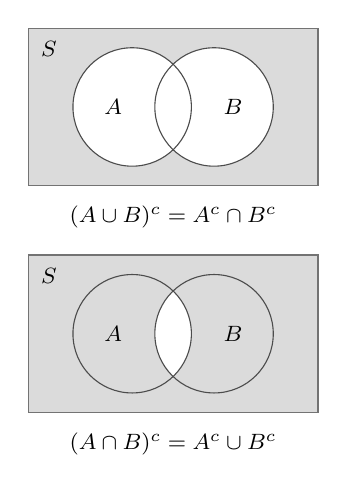
\begin{tikzpicture}[x=0.8cm,y=0.8cm,font=\footnotesize]
  \foreach \offset in {0,-3.6} {
    \begin{scope}[shift={(0,\offset)}]
      \fill[black!14] (0,0) rectangle (4.6,2.5);
    \end{scope}
  }
  % Removing both discs leaves the complement of their union.
  \fill[white] (1.65,1.25) circle[radius=0.94];
  \fill[white] (2.95,1.25) circle[radius=0.94];
  % Removing only the lens leaves the complement of the intersection.
  \begin{scope}[shift={(0,-3.6)}]
    \clip (1.65,1.25) circle[radius=0.94];
    \fill[white] (2.95,1.25) circle[radius=0.94];
  \end{scope}
  \foreach \offset in {0,-3.6} {
    \begin{scope}[shift={(0,\offset)}]
      \draw[black!55] (0,0) rectangle (4.6,2.5);
      \draw[black!70] (1.65,1.25) circle[radius=0.94];
      \draw[black!70] (2.95,1.25) circle[radius=0.94];
      \node at (1.35,1.25) {$A$};
      \node at (3.25,1.25) {$B$};
      \node[anchor=north west] at (0.05,2.45) {$S$};
    \end{scope}
  }
  \node at (2.3,-0.5) {$(A\cup B)^c=A^c\cap B^c$};
  \node at (2.3,-4.1) {$(A\cap B)^c=A^c\cup B^c$};
\end{tikzpicture}

    \caption{The upper shaded region lies outside both sets.
      In the lower panel, only the overlap is excluded. All complements
      are taken within the rectangle $S$.}
    \label{fig:hw01:de-morgan}
  \end{marginfigure}

  \textit{The complement of the union.}
  Suppose that
  \[
    x\in\left(\bigcup_{\gamma\in\Gamma}A_\gamma\right)^c.
  \]
  Then $x\in S$ and $x$ does not belong to the union.
  If $x$ belonged to any $A_\gamma$, it would belong to the union.
  Therefore $x\notin A_\gamma$ for every $\gamma\in\Gamma$.
  Since $x\in S$, this gives $x\in A_\gamma^c$ for every $\gamma$,
  and hence
  \[
    x\in\bigcap_{\gamma\in\Gamma}A_\gamma^c.
  \]

  Conversely, suppose that
  \[
    x\in\bigcap_{\gamma\in\Gamma}A_\gamma^c.
  \]
  Then $x\in S$ and $x\notin A_\gamma$ for every $\gamma\in\Gamma$.
  Thus no member of the family contains $x$, so $x$ does not belong
  to their union. Consequently,
  \[
    x\in\left(\bigcup_{\gamma\in\Gamma}A_\gamma\right)^c.
  \]
  Both inclusions hold, proving the first equality.

  \clearpage

  \textit{The complement of the intersection.}
  Suppose that
  \[
    x\in\left(\bigcap_{\gamma\in\Gamma}A_\gamma\right)^c.
  \]
  Then $x\in S$ and $x$ does not belong to the intersection.
  There must be an index $\gamma_0\in\Gamma$ for which
  $x\notin A_{\gamma_0}$. Otherwise, $x$ would belong to every
  $A_\gamma$ and therefore to their intersection.
  Thus $x\in A_{\gamma_0}^c$, which gives
  \[
    x\in\bigcup_{\gamma\in\Gamma}A_\gamma^c.
  \]

  Conversely, suppose that
  \[
    x\in\bigcup_{\gamma\in\Gamma}A_\gamma^c.
  \]
  Then $x\in A_{\gamma_0}^c$ for at least one index $\gamma_0$.
  Hence $x\in S$ and $x\notin A_{\gamma_0}$.
  Since $x$ fails to belong to this member of the family, it cannot
  belong to the intersection. Thus
  \[
    x\in\left(\bigcap_{\gamma\in\Gamma}A_\gamma\right)^c.
  \]
  Both inclusions hold, proving the second equality.

  If $\Gamma$ is empty, we use the relative conventions
  \[
    \begin{aligned}
      \bigcup_{\gamma\in\varnothing}A_\gamma&=\varnothing,\\
      \bigcap_{\gamma\in\varnothing}A_\gamma&=S.
    \end{aligned}
  \]
  Both identities then follow from $\varnothing^c=S$ and $S^c=\varnothing$.

  Figure~\ref{fig:hw01:de-morgan} illustrates the difference for two sets.
  An element outside their intersection may still belong to one
  of the sets. It simply cannot belong to both.
\end{proof}

\clearpage

\begin{exercise}
\label{ex:hw01:power-set}
List all the elements in the set $\mathcal{P}(\mathcal{P}(\varnothing))$ and verify the cardinality formula.
\end{exercise}

% Transcribed from the right page of IMG_8996.
\begin{proof}[Solution]
  The power set is the set of all subsets. The empty set has exactly
  one subset, itself, so
  \[
    \mathcal{P}(\varnothing)=\{\varnothing\}.
  \]
  Taking the power set once more gives
  \[
    \mathcal{P}(\mathcal{P}(\varnothing))
      =\{\varnothing,\{\varnothing\}\}.
  \]
  Its elements are the empty set and the singleton containing the empty
  set. These are distinct. Since $|\mathcal{P}(\varnothing)|=1$, the
  cardinality formula gives
  \[
    |\mathcal{P}(\mathcal{P}(\varnothing))|
      =2^{|\mathcal{P}(\varnothing)|}=2^1=2.\qedhere
  \]
\end{proof}

\begin{exercise}
\label{ex:hw01:prime-roots}
Let $p=2,3,5,\ldots$ be a prime. Prove that $\sqrt{p}$ is irrational. Can this result be extended to $p^{\frac{1}{k}}$ for any integer $k\geq 2$?
\end{exercise}

% Transcribed from IMG_8997 and the upper left page of IMG_8998.
\begin{proof}[Solution]
  We use Euclid's lemma, which states that if a prime divides a
  product of integers, it divides at least one factor. Applying this
  repeatedly shows that $p\mid a^k$ implies $p\mid a$ for every
  positive integer $k$.

  \textit{The square root.}
  Suppose, for a contradiction, that $\sqrt p\in\Q$. Write
  \[
    \sqrt p=\frac ab,
    \qquad a,b\in\Z,\quad b>0,\quad\gcd(a,b)=1.
  \]
  Squaring gives $a^2=pb^2$, so $p\mid a^2$.
  Euclid's lemma gives $p\mid a$, and we can write $a=pm$
  for some $m\in\Z$. Substituting and cancelling one factor of $p$ gives
  \[
    p^2m^2=pb^2
    \quad\Longrightarrow\quad
    pm^2=b^2.
  \]
  Hence $p\mid b^2$, so Euclid's lemma also gives $p\mid b$.
  The prime $p>1$ therefore divides both $a$ and $b$,
  contradicting $\gcd(a,b)=1$. Thus $\sqrt p$ is irrational.

  \textit{The general $k$th root.}
  Let $k\ge2$ and suppose that $p^{1/k}=a/b$ in lowest terms,
  with $a,b\in\Z$ and $b>0$. Raising both sides to the $k$th
  power gives $a^k=pb^k$. Thus $p\mid a^k$, and Euclid's lemma
  gives $p\mid a$. Writing $a=pm$, we obtain
  \[
    p^km^k=pb^k
    \quad\Longrightarrow\quad
    p^{k-1}m^k=b^k.
  \]
  Since $k-1\ge1$, this shows that $p\mid b^k$, so $p\mid b$.
  Again, $p$ divides both $a$ and $b$, contradicting that the
  fraction is in lowest terms. Therefore $p^{1/k}$ is irrational
  for every integer $k\ge2$.
\end{proof}

\clearpage

\begin{exercise}
\label{ex:hw01:interval-to-reals}
Obtain a bijective map from $(0,1)$ to $\mathbb{R}$.
\end{exercise}

% Transcribed from the lower left and upper right pages of IMG_8998.
\begin{proof}[Solution]
  A map from $A$ to $B$ is a bijection if it is both one-to-one
  and onto. This means that every element of $B$ is the image of
  exactly one element of $A$.
  Figure~\ref{fig:hw01:bijections} contrasts bijections with a map
  that fails both conditions.

  \begin{figure}[h]
    \centering
    % !TEX root = ../../problems/hw01.tex
% Editable reconstruction of the finite-set mapping sketches in IMG_8998.
\begin{tikzpicture}[x=0.9cm,y=0.9cm,>=Stealth,font=\small]
  \foreach \panel/\captiontext in {0/{Bijection},3.8/{Bijection},7.6/{Not a bijection}} {
    \begin{scope}[shift={(\panel,0)}]
      \draw[black!55] (0,0) ellipse[x radius=0.4,y radius=1.05];
      \draw[black!55] (2.1,0) ellipse[x radius=0.4,y radius=1.05];
      \node at (0,1.35) {$A$};
      \node at (2.1,1.35) {$B$};
      \foreach \y in {-0.65,0,0.65} {
        \fill (0,\y) circle[radius=1.5pt];
        \fill (2.1,\y) circle[radius=1.5pt];
      }
      \node[font=\footnotesize] at (1.05,-1.4) {\captiontext};
    \end{scope}
  }
  \foreach \y in {-0.65,0,0.65}
    \draw[->,shorten <=3pt,shorten >=3pt] (0,\y) -- (2.1,\y);
  \draw[->,shorten <=3pt,shorten >=3pt] (3.8,0.65) -- (5.9,-0.65);
  \draw[->,shorten <=3pt,shorten >=3pt] (3.8,0) -- (5.9,0.65);
  \draw[->,shorten <=3pt,shorten >=3pt] (3.8,-0.65) -- (5.9,0);
  \draw[->,shorten <=3pt,shorten >=3pt] (7.6,0.65) -- (9.7,0.65);
  \draw[->,shorten <=3pt,shorten >=3pt] (7.6,0) -- (9.7,0.65);
  \draw[->,shorten <=3pt,shorten >=3pt] (7.6,-0.65) -- (9.7,-0.65);
\end{tikzpicture}

    \caption{The first two maps are bijections. The third map is neither
      one-to-one nor onto. Crossing arrows do not prevent a map from
      being bijective.}
    \label{fig:hw01:bijections}
  \end{figure}

  The tangent function is a bijection from
  $(-\pi/2,\pi/2)$ onto $\R$. To use it on $(0,1)$, we first
  multiply the input by $\pi$ and then subtract $\pi/2$.
  These steps give the composition
  \[
    (0,1)\xrightarrow{\,\times\pi\,}(0,\pi)
      \xrightarrow{\,-\pi/2\,}
      \left(-\frac\pi2,\frac\pi2\right)
      \xrightarrow{\,\tan\,}\R.
  \]
  We can therefore define
  \[
    f(x)=\tan\left(\pi x-\frac\pi2\right),
      \qquad 0<x<1.
  \]
  For $0<x<1$, the angle $\pi x-\pi/2$ lies strictly between
  $-\pi/2$ and $\pi/2$, so $f(x)$ is defined and real.
  We verify bijectivity by giving its inverse. For $y\in\R$, put
  \[
    g(y)=\frac12+\frac{\arctan y}{\pi}.
  \]
  Here $\arctan y$ is the unique angle in $(-\pi/2,\pi/2)$
  whose tangent is $y$. Thus $0<g(y)<1$, and
  \[
    f(g(y))=\tan(\arctan y)=y.
  \]
  This proves that $f$ is onto. Conversely, for $x\in(0,1)$,
  the angle lies in the principal interval, so
  \[
    g(f(x))=\frac12+
      \frac{\arctan(\tan(\pi x-\pi/2))}{\pi}=x.
  \]
  If $f(x_1)=f(x_2)$, applying $g$ gives $x_1=x_2$.
  Therefore $f$ is also one-to-one and hence is a bijection.
  \clearpage

  Figure~\ref{fig:hw01:tangent-overview} shows the central branch of
  $y=\tan t$ in blue and the transformed graph alongside it.
  The horizontal change $x=t/\pi+1/2$ compresses that branch by a
  factor of $1/\pi$ and shifts it to the right by $1/2$.
  Its domain becomes $(0,1)$, while its range remains all of $\R$.

  \begin{figure*}[h]
    \centering
    % !TEX root = ../../problems/hw01.tex
% The tangent overview and its transformed central branch share one figure.
\begin{tikzpicture}[>=Stealth,font=\footnotesize]
  \definecolor{tangentblue}{HTML}{69B4E4}
  \definecolor{tangentwash}{HTML}{EAF6FD}

  \begin{scope}[x=0.62cm,y=0.42cm]
    \fill[tangentwash] (-1.5708,-4.6) rectangle (1.5708,4.6);
    \foreach \boundary in {-2.5,-1.5,1.5,2.5} {
      \draw[dashed,black!30] ({\boundary*pi},-4.6)
        -- ({\boundary*pi},4.6);
    }
    \foreach \boundary in {-0.5,0.5} {
      \draw[dashed,tangentblue] ({\boundary*pi},-4.6)
        -- ({\boundary*pi},4.6);
    }
    \draw[->,black!65] (-8.15,0) -- (8.3,0) node[right] {$t$};
    \draw[->,black!65] (0,-4.85) -- (0,5.05) node[above] {$y$};

    % Sample each branch separately, away from the vertical asymptotes.
    \foreach \period in {-2,-1,1,2} {
      \draw[thick,black!65,<->,domain=-1.347:1.347,samples=121,smooth]
        plot ({\x+\period*pi},{tan(deg(\x))});
    }
    \draw[line width=1.3pt,tangentblue,<->,
      domain=-1.347:1.347,samples=121,smooth]
      plot (\x,{tan(deg(\x))});

    \foreach \period/\ticktext in {-2/{-2\pi},-1/{-\pi},1/{\pi},2/{2\pi}} {
      \draw[black!65] ({\period*pi},0.12) -- ({\period*pi},-0.12);
      \node[below,fill=white,inner sep=2pt]
        at ({\period*pi},-0.14) {$\ticktext$};
    }
    \node[below right,inner sep=2pt] at (0,0) {$0$};
    \foreach \level in {-4,-2,2,4} {
      \draw[black!65] (-0.09,\level) -- (0.09,\level);
      \node[left,inner sep=2pt] at (-0.09,\level) {$\level$};
    }
    \foreach \boundary/\ticktext in {
      -2.5/{-5\pi/2},-1.5/{-3\pi/2},-0.5/{-\pi/2},
      0.5/{\pi/2},1.5/{3\pi/2},2.5/{5\pi/2}} {
      \node[below] at ({\boundary*pi},-4.85) {$\ticktext$};
    }
    \node at (0,-6.4) {$y=\tan t$};
  \end{scope}

  \begin{scope}[shift={(7.05cm,0)},x=2.75cm,y=0.42cm]
    \draw[dashed,black!45] (1,-4.6) -- (1,4.6);
    \draw[->,black!65] (-0.12,0) -- (1.18,0) node[right] {$x$};
    \draw[->,black!65] (0,-4.85) -- (0,5.05) node[above] {$y$};
    % The same parameter t places the selected branch at x=t/pi+1/2.
    \draw[thick,<->,domain=-1.347:1.347,samples=121,smooth]
      plot ({\x/pi+0.5},{tan(deg(\x))});
    \node[below left,fill=white,inner sep=1pt] at (0,0) {$0$};
    \node[below,fill=white,inner sep=2pt] at (1,0) {$1$};
    \node[below right,fill=white,inner sep=2pt] at (0.5,0) {$\tfrac12$};
    \node at (0.5,-6.4) {$y=\tan(\pi x-\pi/2)$};
  \end{scope}
\end{tikzpicture}

    \caption{The left panel highlights the central tangent branch on
      $(-\pi/2,\pi/2)$. The right panel shows this branch after the
      change of input. The vertical asymptotes now occur at $x=0$
      and $x=1$. The horizontal axes use different scales.}
    \label{fig:hw01:tangent-overview}
  \end{figure*}
\end{proof}

\clearpage

\begin{exercise}
\label{ex:hw01:open-to-closed-interval}
Obtain a bijective map from $(0,1)$ to $[0,1]$.
\end{exercise}

% Transcribed from the lower right page of IMG_8998 and left page of IMG_8999.
\begin{proof}[Solution]
  The identity $f(x)=x$ maps $(0,1)$ to itself, but it misses the
  endpoints of $[0,1]$, as shown in Figure~\ref{fig:hw01:identity-map}.
  We can make room for them by moving a countable sequence of points.

  \begin{marginfigure}
    \centering
    % !TEX root = ../../problems/hw01.tex
\begin{tikzpicture}[x=2.9cm,y=2.9cm,>=Stealth,font=\footnotesize]
  \draw[->] (-0.12,0) -- (1.14,0) node[right] {$x$};
  \draw[->] (0,-0.12) -- (0,1.14) node[above] {$y$};
  \draw[thick] (0,0) -- (1,1);
  \draw[densely dotted,black!50] (1,0) -- (1,1) -- (0,1);
  \draw[fill=white] (0,0) circle[radius=1.8pt];
  \draw[fill=white] (1,1) circle[radius=1.8pt];
  \node[below left] at (0,0) {$0$};
  \node[below] at (1,0) {$1$};
  \node[left] at (0,1) {$1$};
  \node[above left] at (0.65,0.65) {$y=x$};
\end{tikzpicture}

    \caption{The identity on $(0,1)$ misses the target values $0$ and $1$.
      Both endpoints of the graph are excluded.}
    \label{fig:hw01:identity-map}
  \end{marginfigure}

  First assign
  \[
    f\left(\frac12\right)=0,
    \qquad f\left(\frac13\right)=1.
  \]
  The values $1/2$ and $1/3$ must now be supplied by other inputs.
  We use $1/4$ and $1/5$ for these values, and then continue shifting
  the reciprocals to fill the resulting gaps. This gives
  \[
    f\left(\frac14\right)=\frac12,\quad
    f\left(\frac15\right)=\frac13,\quad
    f\left(\frac16\right)=\frac14,\quad\ldots
  \]
  Figure~\ref{fig:hw01:reciprocal-shift} illustrates this shift.
  We leave all other points fixed. Define a map $f$ from $(0,1)$
  to $[0,1]$ by
  \[
    f(x)=
    \begin{cases}
      0, & x=\frac12,\\[2pt]
      1, & x=\frac13,\\[2pt]
      \dfrac1{n-2}, & x=\frac1n,\quad n\in\N,\ n\ge4,\\[4pt]
      x, & \text{otherwise}.
    \end{cases}
  \]

  \begin{figure}[h]
    \centering
    % !TEX root = ../../problems/hw01.tex
\begin{tikzpicture}[x=0.92cm,y=1cm,>=Stealth,font=\small]
  \node[anchor=east] at (-0.35,1.2) {$x$};
  \node[anchor=east] at (-0.35,0) {$f(x)$};
  \foreach \pos/\source/\target in {
    0.2/{\frac12}/{0},
    1.55/{\frac13}/{1},
    2.9/{\frac14}/{\frac12},
    4.25/{\frac15}/{\frac13},
    5.6/{\frac16}/{\frac14},
    8.4/{\frac1n}/{\frac1{n-2}}} {
    \node at (\pos,1.2) {$\source$};
    \node at (\pos,0) {$\target$};
    \draw[->] (\pos,0.86) -- (\pos,0.35);
  }
  \node at (7,1.2) {$\cdots$};
  \node at (7,0) {$\cdots$};
  \node at (9.55,1.2) {$\cdots$};
  \node at (9.55,0) {$\cdots$};
\end{tikzpicture}

    \caption{The reciprocal sequence is shifted to accommodate both
      endpoints. Every point outside this sequence remains fixed.}
    \label{fig:hw01:reciprocal-shift}
  \end{figure}

  To check bijectivity, put
  \[
    S=\left\{\frac1n\mid n\in\N,\ n\ge2\right\}.
  \]
  The cases in the definition are disjoint and cover $(0,1)$.
  Every output lies in $[0,1]$, so the function is well-defined.

  Among the inputs in $S$, only $1/2$ maps to $0$, and only $1/3$
  maps to $1$. For each integer $m\ge2$, solving $1/(n-2)=1/m$
  gives the unique input $1/(m+2)$. Thus $f$ maps $S$ bijectively
  onto $S\cup\{0,1\}$.

  On $(0,1)\setminus S$, the map is the identity, with image
  $(0,1)\setminus S$. This image is disjoint from $S\cup\{0,1\}$,
  so no fixed point can give a second preimage for a value already
  supplied by the reciprocal sequence. Together the two images
  cover $[0,1]$. Every target value therefore has exactly one
  preimage, proving that $f$ is a bijection.
\end{proof}

\clearpage

\begin{exercise}
\label{ex:hw01:transcendental-cardinality}
Let $\aleph_0$ and $\aleph$ denote the cardinalities of $\mathbb{N}$ and $\mathbb{R}$ respectively. Recall that the Continuum Hypothesis (CH) states that there is no cardinality between $\aleph_0$ and $\aleph$. Use CH to prove that the set of transcendental numbers, $\mathbb{T}$, has the same cardinality $\aleph$ as that of $\mathbb{R}$.
\end{exercise}

% Completed from the argument on the right page of IMG_8999.
\begin{proof}[Solution]
  Let $\mathbb{A}$ be the set of real algebraic numbers and
  $\mathbb{T}$ the set of real transcendental numbers. An algebraic
  number is a root of a nonzero polynomial with integer coefficients;
  a transcendental number is not such a root. Hence
  \[
    \R=\mathbb{A}\cup\mathbb{T},
    \qquad\mathbb{A}\cap\mathbb{T}=\varnothing.
  \]
  First, we show that $\mathbb{A}$ is countable. For each $n\ge1$,
  consider the nonzero polynomials
  \[
    P(X)=c_0+c_1X+\cdots+c_nX^n,
    \qquad c_j\in\Z,\quad |c_j|\le n.
  \]
  Each of the $n+1$ coefficients has $2n+1$ possible values, so
  there are at most $(2n+1)^{n+1}$ such polynomials.
  A nonzero polynomial of degree at most $n$ has at most $n$
  distinct real roots. Thus the set $F_n$ of all their real roots
  is finite.

  Every algebraic number is a root of a nonzero integer polynomial.
  Taking $n$ at least as large as its degree and the absolute values
  of all its coefficients places that root in $F_n$.
  Conversely, every root in $F_n$ is algebraic. Hence
  \[
    \mathbb{A}=\bigcup_{n=1}^{\infty}F_n.
  \]
  Within each finite set $F_n$, list the roots in increasing order.
  Read these finite lists in the order $F_1,F_2,\ldots$, skipping
  repeated roots. Each root is reached after finitely many steps.
  This proves that $\mathbb{A}$ is countable. Every $n\in\N$
  is a root of $X-n$, so $\N\subseteq\mathbb{A}$. Thus
  $\mathbb{A}$ is infinite, and $|\mathbb{A}|=\aleph_0$.

  \begin{marginfigure}
    \centering
    % !TEX root = ../../problems/hw01.tex
\begin{tikzpicture}[x=1cm,y=1cm,>=Stealth,font=\footnotesize]
  \draw[->,black!55] (0,0) -- (3.8,0);
  \draw[black!65,fill=white] (0.25,0) circle[radius=2.5pt];
  \fill (3.45,0) circle[radius=3pt];
  \node[below=6pt] at (0.25,0) {$\aleph_0$};
  \node[below=6pt] at (3.15,0) {$|\mathbb{T}|=\aleph$};
  \node[above=8pt,align=center] at (1.85,0)
    {No intermediate\\cardinality under CH};
\end{tikzpicture}

    \caption{CH excludes intermediate cardinalities. Since
      $\mathbb{T}$ is uncountable and contained in $\R$, its cardinality
      must equal $\aleph$.}
    \label{fig:hw01:continuum-gap}
  \end{marginfigure}

  Now suppose that $\mathbb{T}$ were countable. Then
  $\R=\mathbb{A}\cup\mathbb{T}$ would be a union of two countable
  sets and therefore countable. This contradicts the uncountability
  of $\R$. Hence $\mathbb{T}$ is uncountable. Since
  $\mathbb{T}\subseteq\R$, we have
  \[
    \aleph_0<|\mathbb{T}|\le|\R|=\aleph.
  \]
  By CH there is no cardinality strictly between $\aleph_0$ and
  $\aleph$, as illustrated in Figure~\ref{fig:hw01:continuum-gap}.
  The lower endpoint is already excluded, so the only possibility is
  \[
    |\mathbb{T}|=\aleph.\qedhere
  \]
\end{proof}

\clearpage

\begin{exercise}
\label{ex:hw01:linear-independence}
Let $\tau$ be a transcendental number whose existence is proven already. Show that for any $n\in\mathbb{N}$, the numbers
\[
    \tau,\ldots,\tau^n
\]
are linearly independent over the field $\mathbb{Q}$.

That is, if there are $r_1,\ldots,r_n\in\mathbb{Q}$ such that
\[
    r_1\tau+\cdots+r_n\tau^n=0,
\]
then $r_1=\cdots=r_n=0$.

(In the language of Linear Algebra, this result indicates that the set $\mathbb{R}$ viewed as a vector space over $\mathbb{Q}$ is infinitely dimensional.)
\end{exercise}

\begin{proof}[Solution]
  Suppose that
  \[
    r_1\tau+\cdots+r_n\tau^n=0,
    \qquad r_1,\ldots,r_n\in\Q.
  \]
  We want to show that every coefficient is zero. Suppose, for a
  contradiction, that at least one $r_j\ne0$.

  Write $r_j=a_j/b_j$, where $a_j\in\Z$ and $b_j\in\N$.
  Put $D=b_1\cdots b_n>0$. We multiply through by $D$ to clear
  all the denominators and obtain
  \[
    (Dr_1)\tau+\cdots+(Dr_n)\tau^n=0.
  \]
  Each $Dr_j$ is an integer, and at least one is nonzero since
  $D\ne0$. Therefore
  \[
    P(X)=(Dr_1)X+\cdots+(Dr_n)X^n
  \]
  is a nonzero polynomial with integer coefficients satisfying
  $P(\tau)=0$. This would make $\tau$ algebraic, contradicting
  the assumption that it is transcendental.

  Thus $r_1=\cdots=r_n=0$. Since $n$ was arbitrary, the numbers
  $\tau,\ldots,\tau^n$ are linearly independent over $\Q$ for every
  $n\in\N$.
  \marginnote{Including a constant term does not change the argument.
    Thus $1,\tau,\ldots,\tau^n$ are also linearly independent over $\Q$.}
\end{proof}

\clearpage

\begin{exercise}
\label{ex:hw01:square-cardinality}
Show that
\[
    |(0,1)\times(0,1)|=|(0,1)|=\aleph.
\]
(\textit{Corrected hint.} For each number in $(0,1)$, choose the decimal
expansion that is not eventually all $9$s. We can then write
\[
    x\in(0,1),\quad x=0.x_1x_2\cdots,\quad
    x_i\in\{0,\ldots,9\},\quad i=1,2,\ldots.
\]
Then define a map from $(0,1)\times(0,1)$ to $(0,1)$ by
\[
    (x,y)=(0.x_1x_2\cdots,0.y_1y_2\cdots)
    \mapsto (0.x_1y_1x_2y_2\ldots)=z\in(0,1).
\]
Show that this map is injective, then use injections in both directions.)
\end{exercise}

\begin{proof}[Solution]
  Put $I=(0,1)$. For each number in $I$, we choose the unique
  decimal expansion that is not eventually all $9$s.
  For example, we write one half as $0.5000\ldots$ instead of
  $0.4999\ldots$. Each digit may be any of $0,1,\ldots,9$.

  For $x=0.x_1x_2\ldots$ and $y=0.y_1y_2\ldots$, define
  \[
    F(x,y)=0.x_1y_1x_2y_2\ldots.
  \]
  Figure~\ref{fig:hw01:decimal-interleaving} shows how the odd
  positions record $x$ and the even positions record $y$.

  \begin{figure*}[h]
    \centering
    % !TEX root = ../../problems/hw01.tex
\begin{tikzpicture}[x=1cm,y=1cm,>=Stealth,font=\small]
  \node[anchor=east] at (-0.75,1.25) {$x=0.$};
  \node[anchor=east] at (-0.75,0) {$F(x,y)=0.$};
  \node[anchor=east] at (-0.75,-1.25) {$y=0.$};
  \foreach \index in {1,2,3,4} {
    \pgfmathsetmacro{\oddpos}{3.0*(\index-1)}
    \pgfmathsetmacro{\evenpos}{\oddpos+1.5}
    \node[text=black] (x\index) at (\oddpos,1.25) {$x_{\index}$};
    \node[text=black] (y\index) at (\evenpos,-1.25) {$y_{\index}$};
    \node[fill=black!6,minimum width=0.65cm,minimum height=0.5cm]
      (odd\index) at (\oddpos,0) {$x_{\index}$};
    \node[fill=black!12,minimum width=0.65cm,minimum height=0.5cm]
      (even\index) at (\evenpos,0) {$y_{\index}$};
    \draw[->,black!65] (x\index.south) -- (odd\index.north);
    \draw[->,black!65] (y\index.north) -- (even\index.south);
  }
  \foreach \height in {-1.25,0,1.25}
    \node at (12.0,\height) {$\cdots$};
\end{tikzpicture}

    \caption{Interleaving keeps both digit sequences. Read the odd
      positions to recover $x$, and the even positions to recover $y$.}
    \label{fig:hw01:decimal-interleaving}
  \end{figure*}

  \clearpage

  We first check that this construction gives a number in $I$.
  The output digits cannot be eventually all $9$s. Otherwise,
  both input expansions would also be eventually all $9$s,
  contradicting our choice of decimal expansions.

  Since $x>0$, at least one of its digits is nonzero. This digit
  occurs in an odd position of the output, so $F(x,y)>0$.
  The output is less than $1$ because its digits are not all $9$s.
  Therefore $F(x,y)\in I$, and its displayed decimal expansion
  follows our convention.

  If $F(x,y)=F(u,v)$, uniqueness of the digits gives $x_j=u_j$
  and $y_j=v_j$ for every $j$. Hence $x=u$ and $y=v$, so $F$
  is one-to-one.

  However, $F$ is not onto, despite the claim in the original hint.
  To see this, consider $z=0.101010\ldots\in I$.
  If $F(x,y)=z$, the even digits would force $y=0.000\ldots=0$.
  This is impossible because $0\notin I$, so $z$ has no preimage.

  We therefore use an injection in the reverse direction as well.
  Define a map $G$ from $I$ to $I\times I$ by
  \[
    G(t)=\left(t,\frac12\right).
  \]
  Both coordinates lie in $I$, so the map is well-defined.
  If $G(t)=G(s)$, equality of the first coordinates gives $t=s$.
  Hence $G$ is one-to-one.

  The Cantor--Schr\"oder--Bernstein theorem says that injections
  in both directions imply the existence of a bijection.
  Applying it to $F$ and $G$ gives $|I\times I|=|I|$.
  By Exercise~\ref{ex:hw01:interval-to-reals}, $|I|=|\R|=\aleph$.
  Therefore
  \[
    |(0,1)\times(0,1)|=|(0,1)|=\aleph.\qedhere
  \]
\end{proof}

\begin{exercise}
\label{ex:hw01:irrational-roots}
Show that if $a>0$ is irrational, so is the $k$th root of $a$, $a^{\frac{1}{k}}$, for any $k\in\mathbb{N}$.
\end{exercise}

\begin{proof}[Solution]
  Let $k\ge1$. Suppose, for a contradiction, that $a^{1/k}$ is
  rational. Then
  \[
    a^{1/k}=\frac pq,
    \qquad p,q\in\Z,\quad q\ne0.
  \]
  Raising both sides to the $k$th power gives
  \[
    a=\left(\frac pq\right)^k=\frac{p^k}{q^k}\in\Q,
  \]
  since $p^k,q^k\in\Z$ and $q^k\ne0$. This contradicts the
  assumption that $a$ is irrational. Therefore $a^{1/k}$ is
  irrational for every $k\in\N$.
\end{proof}

\clearpage

\begin{exercise}
\label{ex:hw01:countable-union}
Let $A_n$ be a set such that $|A_n|=\aleph_0$ for $n=1,2,\ldots$. Prove $|A|=\aleph_0$ where
\[
    A=\bigcup_{n=1}^{\infty} A_n.
\]
\end{exercise}

\begin{proof}[Solution]
  Since each $A_n$ is countably infinite, there exists a bijection
  from $\N$ to $A_n$. Using the axiom of countable choice, select
  one such bijection for each $n$. This gives a list without
  repetition within each row, which we write as
  \[
    A_n=\{a_{n,1},a_{n,2},a_{n,3},\ldots\}.
  \]
  Put these lists into rows. Reading one whole row first would
  never reach the next row. Instead, follow successive diagonals
  $n+m=2,3,\ldots$, alternating direction as in
  Figure~\ref{fig:hw01:diagonal-enumeration}. This gives
  \[
    a_{1,1},\ a_{1,2},\ a_{2,1},\ a_{3,1},
    \ a_{2,2},\ a_{1,3},\ a_{1,4},\ldots.
  \]

  \begin{figure}[h]
    \centering
    % !TEX root = ../../problems/hw01.tex
\begin{tikzpicture}[x=1.85cm,y=0.72cm,>=Stealth,font=\small]
  \foreach \col in {1,2,3,4} {
    \node[font=\footnotesize] at (\col,0.75) {$m=\col$};
    \node at (\col,-4) {$\vdots$};
  }
  \foreach \row in {1,2,3,4} {
    \node[anchor=east] at (0.4,{1-\row}) {$A_{\row}$};
    \node at (4.75,{1-\row}) {$\cdots$};
    \foreach \col in {1,2,3,4}
      \node (a\row\col) at (\col,{1-\row}) {$a_{\row,\col}$};
  }
  \node at (4.75,-4) {$\ddots$};
  \foreach \from/\to in {11/12,12/21,21/31,31/22,22/13,
    13/14,14/23,23/32,32/41} {
    \draw[->,black!60,line width=0.85pt,shorten <=2pt,shorten >=2pt]
      (a\from) -- (a\to);
  }
  \draw[->,black!60,line width=0.85pt]
    (a41.south) -- (1,-3.7);
\end{tikzpicture}

    \caption{Follow the arrows along diagonals of constant $n+m$.
      Every entry is reached after finitely many steps.}
    \label{fig:hw01:diagonal-enumeration}
  \end{figure}

  Each diagonal is finite, and each $a_{n,m}$ has only finitely
  many diagonals before its own. Hence every entry is eventually
  reached. Every element of $A$ occurs in some row, so this sequence
  contains all of $A$.

  The sets may overlap. Skip any value already listed, keeping only
  its first occurrence. Every element has a first occurrence at
  a finite position, so none is lost by this procedure. The
  retained list contains each element of $A$ exactly once.
  Since $A_1\subseteq A$ is infinite, the retained list is also
  infinite. Numbering its entries in order gives a bijection
  from $\N$ to $A$. Therefore
  \[
    |A|=\aleph_0.\qedhere
  \]
\end{proof}

\end{document}
